% !TeX program = xelatex
\documentclass[11pt,a4paper]{ctexart}
\usepackage{amsmath,amssymb,mathtools}
\usepackage{booktabs,tabularx,array,longtable}
\usepackage{graphicx,float,xcolor,geometry,hyperref,enumitem,listings}
\usepackage[most]{tcolorbox}
\geometry{left=2.15cm,right=2.15cm,top=2.25cm,bottom=2.25cm}
\hypersetup{colorlinks=true,linkcolor=blue!55!black,urlcolor=blue!55!black,citecolor=blue!55!black}
\graphicspath{{assets/}{../results/figures/}}
\setlength{\parindent}{2em}
\setlength{\parskip}{0.25em}
\setlist[itemize]{itemsep=0.25em,topsep=0.35em}
\setlist[enumerate]{itemsep=0.25em,topsep=0.35em}
\definecolor{ZJUBlue}{RGB}{0,63,136}
\definecolor{ZJUGreen}{RGB}{0,125,117}
\definecolor{LightBlue}{RGB}{237,245,253}
\definecolor{LightGreen}{RGB}{235,248,246}
\definecolor{LightOrange}{RGB}{255,246,231}
\newcommand{\key}[1]{\textcolor{ZJUBlue}{\textbf{#1}}}
\newcommand{\good}[1]{\textcolor{ZJUGreen}{\textbf{#1}}}
\newcommand{\KL}{D_{\mathrm{KL}}}
\newtcolorbox{takeaway}{colback=LightBlue,colframe=ZJUBlue,title=一句话结论,fonttitle=\bfseries}
\newtcolorbox{warningbox}{colback=LightOrange,colframe=orange!70!black,title=汇报边界,fonttitle=\bfseries}
\newtcolorbox{intuition}{colback=LightGreen,colframe=ZJUGreen,title=直觉,fonttitle=\bfseries}
\lstset{basicstyle=\ttfamily\small,backgroundcolor=\color{gray!7},frame=single,breaklines=true,columns=fullflexible,keepspaces=true}
\title{《Optimal Pricing for Data-Augmented AutoML Marketplaces》\\\large RQ1 与 RQ3 中期汇报个人讲义}
\author{课程大作业 C.3 · 实验复现部分}
\date{2026 年 7 月 17 日}

\begin{document}
\maketitle
\begin{abstract}
本文只服务于中期汇报中负责 RQ1 和 RQ3 的同学。RQ1 研究平台能否以较少模型训练找到高质量的“数据增强--模型”组合，对应论文 Algorithm~2 的 Data-Bandit；RQ3 研究平台能否从买家的停止轮次学习未知类型先验，对应 Algorithm~1 的平滑贝叶斯学习，并依赖 Algorithm~3 的最优停止行为。本讲义依次解释研究问题、算法直觉与公式、原论文实验、项目缩减复现、指标和结果解读，最后给出讲述顺序、常见追问与准确回答。原文 Figure~3/5 与本项目结果必须分开表述：前者来自论文，后者分别使用公开 UCI 数据和透明合成环境，目标是复现算法语义和定性现象，不是逐点还原原图。
\end{abstract}
\tableofcontents
\newpage

\section{先把两项 RQ 放回整篇论文}
论文市场包含四个连续环节：
\[
\text{外部数据增强与模型发现}
\longrightarrow \text{性能轨迹 }(q_1,\ldots,q_T)
\longrightarrow \text{买家停止/购买}
\longrightarrow \text{平台学习并更新价格}.
\]

\begin{table}[H]
\centering
\caption{RQ、问题、算法和实验之间的对应关系。}
\begin{tabularx}{\textwidth}{>{\bfseries\raggedright\arraybackslash}p{0.09\textwidth}>{\raggedright\arraybackslash}p{0.25\textwidth}>{\raggedright\arraybackslash}p{0.25\textwidth}>{\raggedright\arraybackslash}X}
\toprule
& 研究问题 & 对应算法 & 实验回答方式\\
\midrule
RQ1 & 能否快速找到高质量的数据增强--模型组合？ & Algorithm 2：Metam 风格增强搜索 + Exp3 模型选择 & 比较 Data-Bandit、Data-All、Data-Alt、AutoML 的效用--预算曲线\\
RQ3 & 能否仅从停止时间学到真实买家类型分布？ & Algorithm 1：停止似然、Bayes 后验、学习率平滑；Algorithm 3 提供停止行为 & 比较不同先验、学习率和批量下的 KL 收敛速度与波动\\
\bottomrule
\end{tabularx}
\end{table}

\begin{takeaway}
RQ1 解决“平台怎样产生好的性能轨迹”，RQ3 解决“平台怎样利用买家在轨迹上的停止行为学习市场”。RQ1 提供轨迹，最优停止产生观测，RQ3 再从观测反推买家分布。
\end{takeaway}

\section{RQ1：能否高效发现增强--模型组合}
\subsection{研究问题究竟在问什么}
假设平台有候选增强集合 $\mathcal P$ 和模型集合 $\mathcal M$。穷举所有增强子集和模型，需要训练
\[
O\!\left(2^{|\mathcal P|}|\mathcal M|\right)
\]
个模型。即使用 Metam 等方法把增强搜索缩减到 $O(\log|\mathcal P|)$ 轮，如果每轮仍训练全部 $|\mathcal M|$ 个模型，训练数仍是 $O(|\mathcal M|\log|\mathcal P|)$。因此 RQ1 同时问：固定预算下谁更早找到高效用组合、达到接近 oracle 的性能需要多少训练，以及少训练是否牺牲最终性能。

\begin{intuition}
如果一次增强有六个模型，Data-All 会立即花六次训练把这个增强测透；Data-Bandit 先花一次训练判断它是否值得继续。省下来的预算可以探索更多增强。它优化的是\textbf{搜索过程中的样本效率}，不是承诺每个有限预算终点都严格优于穷举。
\end{intuition}

\subsection{Algorithm 2：Data-Bandit 的两层结构}
Algorithm~2 把“选增强”和“选模型”拆成两层：增强层从外部数据中提出当前最值得测试的增强 $T_i$；模型层把每个 $M\in\mathcal M$ 看作 Exp3 的一只臂，每轮只抽取一只臂训练。

设模型权重为 $w_i(M)$、探索系数为 $\gamma$，第 $i$ 轮抽模型的概率为
\begin{equation}
p_i(M)=(1-\gamma)\frac{w_i(M)}{\sum_{M'}w_i(M')}+\frac{\gamma}{|\mathcal M|}.
\label{eq:exp3-prob}
\end{equation}
第一项偏向历史表现好的模型，第二项保证每个模型至少有 $\gamma/|\mathcal M|$ 的探索概率。抽到 $M_i$ 后，在 $D_{\mathrm{in}}\Join T_i$ 上训练并得到奖励 $r_i\in[0,1]$。由于只观察被抽中模型，使用重要性加权
\[
\widehat r_i(M_i)=\frac{r_i}{p_i(M_i)},
\]
再更新
\begin{equation}
w_{i+1}(M_i)=w_i(M_i)\exp\!\left(\frac{\gamma\widehat r_i(M_i)}{|\mathcal M|}\right).
\label{eq:exp3-update}
\end{equation}

\begin{intuition}
若一个模型被很小概率抽到却取得高奖励，$r_i/p_i(M_i)$ 会较大，系统会迅速提高其权重。这个校正让“只观察一只臂”仍能纠正不同模型被观察频率不同造成的偏差。
\end{intuition}

\subsection{为什么是 Exp3}
每轮输入数据因增强 $T_i$ 改变，同一模型的奖励分布并非固定不变。原文将其视为更接近对抗式 bandit 的环境；Exp3 不依赖固定随机奖励分布，并通过显式探索处理变化的数据。算法还具有 anytime 性质：每轮都产生当前性能 $q_i$，买家可以随时停止，正好与论文的停止定价机制衔接。

\subsection{四种方法一定要区分清楚}
\begin{description}[style=nextline,leftmargin=2.7cm]
\item[Data-Bandit] 每个增强只抽样训练一个模型，用 Exp3 更新模型权重。
\item[Data-All] 对每个候选增强训练全部模型；单个增强判断充分，但预算消耗最快。
\item[Data-Alt] 原文固定一个高效低成本模型测试增强，并周期性在当前最佳增强上运行 AutoML。项目中用固定线性模型筛增强，每三个增强周期性测试全部六个模型，保留相同预算语义。
\item[AutoML] 不搜索外部数据，只在原始输入数据上搜索模型。
\end{description}

\subsection{原论文 RQ1 实验与结论}
原文使用约 69K 个 NYC Open Data 数据集组成的数据池，约含 30M 列、3B 行；在 1000 个分类/回归输入任务上平均。例子包括学校考试成绩预测和交通碰撞数量预测。模型库包含 Random Forest、XGBoost、Neural Network 等。

\begin{figure}[H]
\centering
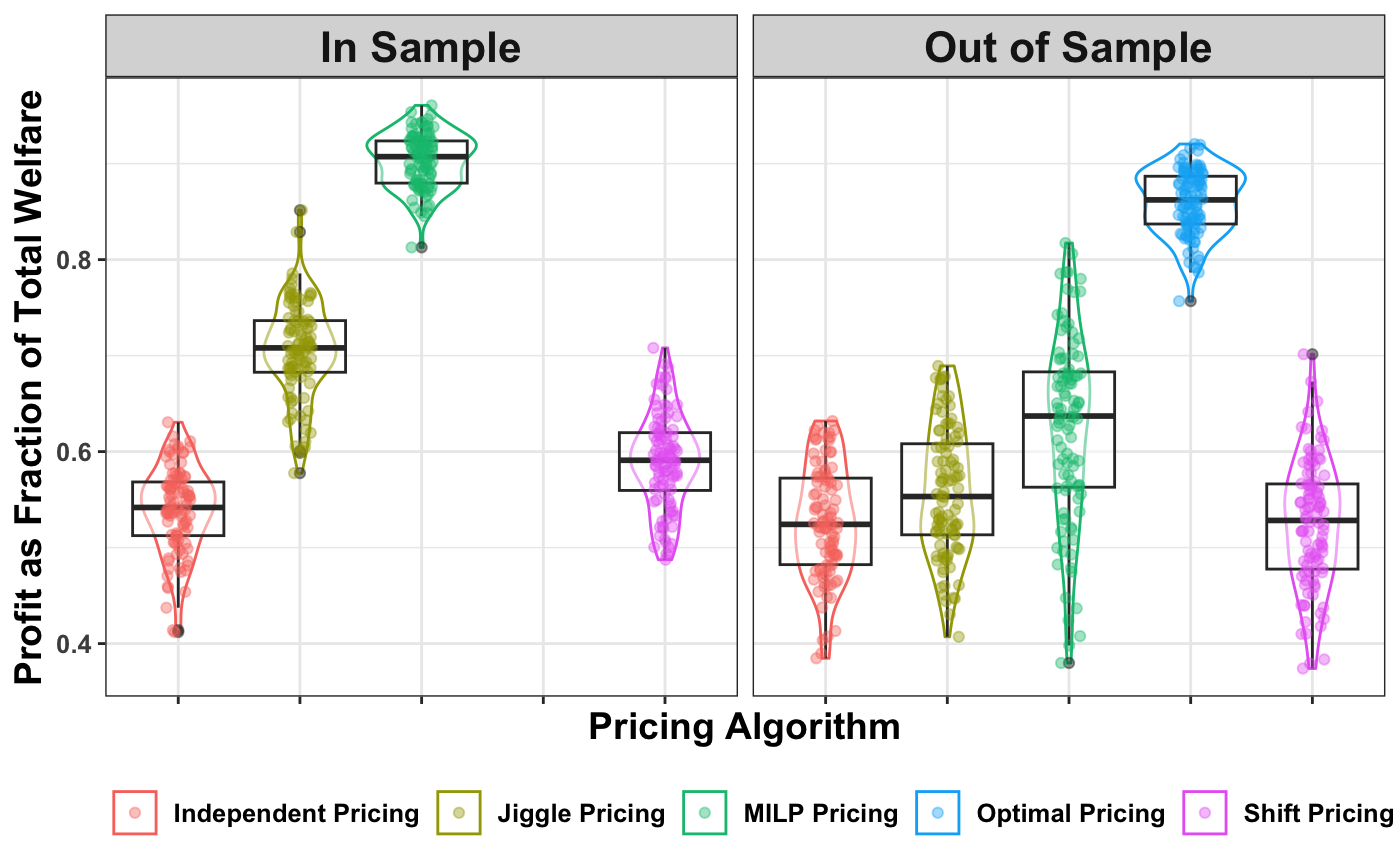
\includegraphics[width=0.76\textwidth]{paper_rq1_figure3.png}
\caption{原论文 Figure 3 的图像部分。横轴是搜索时间，纵轴是效用；右图还报告增强数量。}
\label{fig:paper-rq1}
\end{figure}

原文报告：分类上 Data-Bandit 平均效用超过 0.85，次优基线略高于 0.7，AutoML 约 0.55；回归上在固定搜索时间点，Data-Bandit 也高于基线；大多数任务使用的增强数少于 10。

\begin{warningbox}
原文图的横轴是秒，依赖机器、TPOT 和 NYC 数据池；本项目图的横轴是模型训练次数。两者都刻画搜索成本，但不能把本项目数字与原文时间轴逐点比较。
\end{warningbox}

\subsection{本项目怎样缩减复现 RQ1}
原始 NYC 任务、Metam 配置和完整代码不可得，因此项目使用公开 UCI Wine Quality 构造可连接增强任务：
\begin{itemize}
  \item 红/白葡萄酒各做 15 次固定种子重复；分类与回归分别 30 个任务，共 60 个任务；
  \item 每个任务抽取 1200 条记录，按 60\%/20\%/20\% 分为训练、验证和测试；
  \item 前两个特征作为基础数据，其余九个特征依训练集相关性排序，逐个作为外部增强加入；
  \item 分类目标是质量是否至少为 6，效用为准确率；回归效用为
  \[
  U=\frac{1}{1+\mathrm{RMSE}/\mathrm{Std}(y)};
  \]
  \item 六个模型为四种正则强度的线性模型、二次特征模型和随机 ReLU 特征模型；
  \item 每种方法最多允许 60 次模型训练；验证集负责搜索，测试集只报告由验证集选出的 incumbent，避免测试泄漏。
\end{itemize}

\subsection{四个指标怎么读}
令第 $b$ 次训练后当前最好方案的测试效用为 $U_b$，总预算为 $B=60$。
\begin{enumerate}
  \item \key{最终效用} $U_B$：回答“预算全部用完后谁最好”。
  \item \key{发现曲线 AUC}：
  \[
  \mathrm{AUC}=\frac{1}{B}\sum_{b=1}^{B}U_b.
  \]
  项目输出字段沿用 \texttt{normalized\_auc}；“归一化”指除以预算长度，不是除以 oracle。它回答“整个搜索过程中谁更早找到好方案”。
  \item \key{达到 95\% oracle 增益所需训练数}：令基础效用为 $U_0$、验证选择 oracle 的测试效用为 $U^*$，目标阈值是
  \[
  U_0+0.95\max\{0,U^*-U_0\}.
  \]
  首次达到阈值的训练次数越少越好；未达到记为 $B+1=61$。
  \item \key{配对 bootstrap 区间}：同一个任务上计算 Bandit 与基线的 AUC 差，再对任务重采样。区间不跨 0 才支持平均差异显著不为 0。
\end{enumerate}

\subsection{复现结果及准确解读}
\begin{figure}[H]
\centering
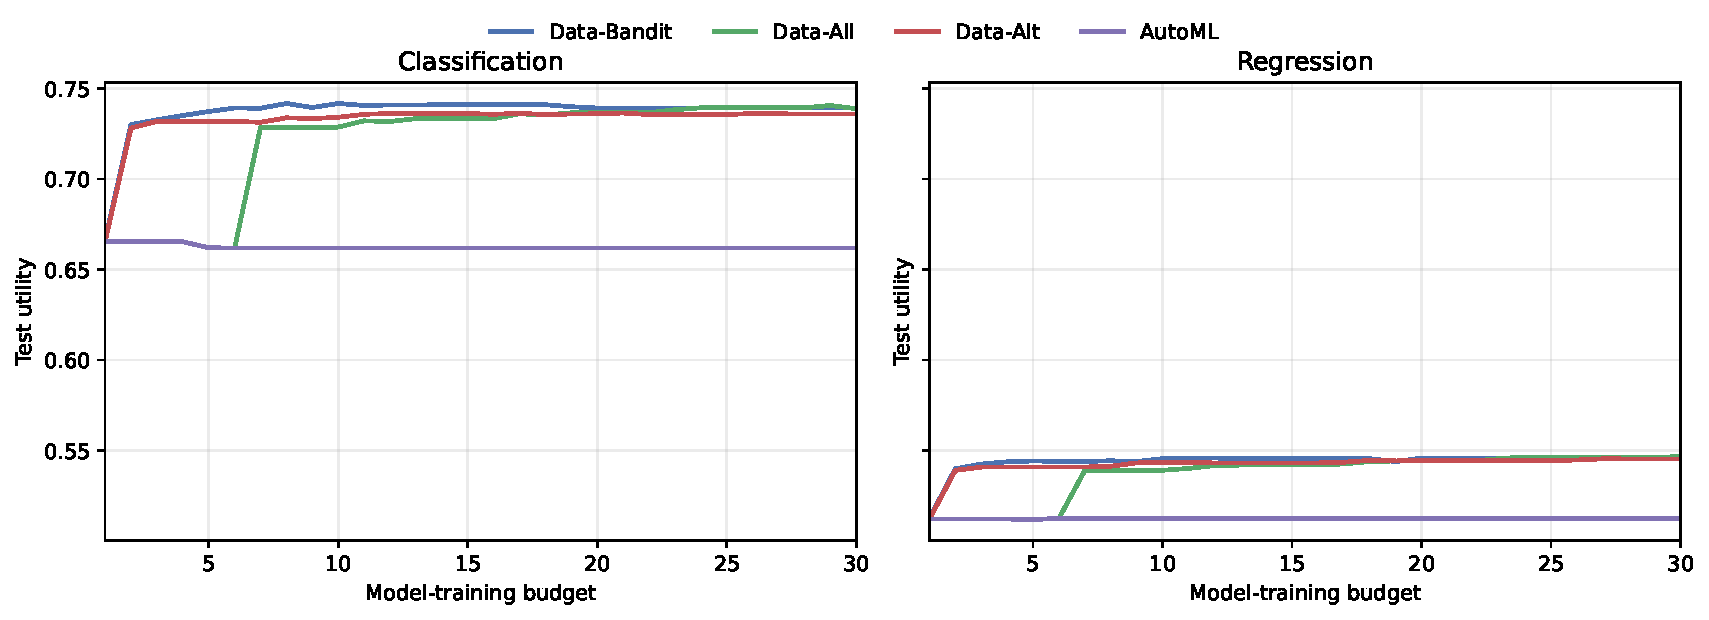
\includegraphics[width=0.98\textwidth]{rq1_discovery.pdf}
\caption{RQ1 缩减复现。前两图为分类/回归 incumbent 测试效用，第三图为达到 95\% oracle 增益所需训练数。}
\label{fig:rq1-reproduction}
\end{figure}

\begin{table}[H]
\centering
\caption{Data-Bandit 相比 Data-All 的核心结果。}
\begin{tabular}{lccc}
\toprule
任务 & AUC 配对差 & 95\% bootstrap 区间 & 95\% 增益训练节省\\
\midrule
分类 & $+0.00794$ & $[0.00340,\,0.01220]$ & 30.3\%\\
回归 & $+0.00335$ & $[0.00185,\,0.00481]$ & 27.5\%\\
\bottomrule
\end{tabular}
\end{table}

正确结论分三层：
\begin{enumerate}
  \item \good{搜索过程更高效：}Bandit 相比 Data-All 的 AUC 配对区间均不跨 0，并以更少训练达到 95\% oracle 增益。
  \item \key{完整预算终点不是 Bandit 最好：}分类终点为 Data-All 0.74083、Bandit 0.73931；回归为 0.54715、0.54590，差距约 0.0012--0.0015。
  \item \key{对 Data-Alt 只能说相当：}分类/回归 AUC 差的区间都跨 0，不能声称 Bandit 显著更优。
\end{enumerate}

\begin{takeaway}
RQ1 复现支持“Data-Bandit 更早找到接近 oracle 的方案”，但不支持“任意预算和任意基线下都最好”。这恰好体现发现算法的目标：在买家可能随时停止的市场里，提高前期搜索效率。
\end{takeaway}

\subsection{RQ1 代码与复现入口}
\begin{itemize}
  \item 算法与数据：\path{src/automl_market/discovery.py}
  \item 实验脚本：\path{scripts/run_rq1.py}
  \item 逐任务结果：\path{results/tables/rq1_task_results.csv}
  \item 配对比较：\path{results/tables/rq1_paired_comparisons.csv}
\end{itemize}
\begin{lstlisting}[language=bash]
conda activate automl-market
make rq1
\end{lstlisting}

\section{RQ3：能否从停止时间学习买家先验}
\subsection{为什么停止时间包含类型信息}
买家类型 $\theta$ 决定估值曲线 $v^\theta(q)$。面对同一价格和性能演化，高估值或更有耐心的类型可能愿意继续等待，低估值类型可能更早停止。因此停止轮次 $y\in\{1,\ldots,T\}$ 是可观察的行为信号。平台看不到买家类型，但如果已知每类买家的停止时间分布，就能用 Bayes 公式反推类型概率。

\begin{intuition}
把停止时间想成医学检测结果：类型是隐藏状态，停止轮次是观测。观测不直接等于类型，但不同类型产生该观测的概率不同，所以可以更新信念。
\end{intuition}

\subsection{Algorithm 1 的两阶段结构}
\paragraph{阶段一：预计算停止似然。}
给定价格 $x$、转移矩阵和类型 $\theta_i$，用最优停止 DP（Algorithm~3/Proposition~4.1）求行为策略，再计算
\[
L_i(y)=\Pr(Y=y\mid \theta_i,x),\qquad y=1,\ldots,T.
\]

\paragraph{阶段二：根据市场观测更新先验。}
当前估计先验为 $\mu^{(t)}$。观察一位买家在 $y^{(t)}$ 停止后，类型后验为
\begin{equation}
w^{(t)}(\theta_i)=\frac{L_i(y^{(t)})\mu^{(t)}(\theta_i)}{\sum_jL_j(y^{(t)})\mu^{(t)}(\theta_j)}.
\label{eq:bayes}
\end{equation}
论文不是直接令新先验等于后验，而是平滑更新：
\begin{equation}
\mu^{(t+1)}=(1-\eta_t)\mu^{(t)}+\eta_tw^{(t)}.
\label{eq:smooth}
\end{equation}
若一轮观察 $b$ 位买家，则先平均各自后验 $\bar w^{(t)}=b^{-1}\sum_{k=1}^bw_k^{(t)}$，再用 $\bar w^{(t)}$ 更新。

\subsection{三种学习率为什么表现不同}
\begin{table}[H]
\centering
\caption{学习率的速度--稳定性含义。}
\begin{tabularx}{\textwidth}{>{\bfseries}p{0.18\textwidth}p{0.29\textwidth}X}
\toprule
学习率 & 行为 & 预期现象\\
\midrule
$1/(t+1)$ & 很快衰减到接近 0 & 后期非常稳定，但早期误差若未纠正，之后更新能力不足\\
$1/\sqrt t$ & 衰减慢于调和学习率 & 持续吸收数据，通常兼顾收敛速度和稳定性\\
$1/2$ & 始终不衰减 & 对新批次反应最快，但抽样噪声一直进入估计，尾部振荡明显\\
\bottomrule
\end{tabularx}
\end{table}
批量 $b$ 越大，平均后验中的抽样噪声越小，所以尤其能稳定常数学习率；代价是每次更新需要更多买家观测。

\subsection{可识别性：RQ3 最重要的前提}
若两个类型满足
\[
\Pr(Y=y\mid\theta_i,x)=\Pr(Y=y\mid\theta_j,x)
\quad\text{对所有 }y\text{ 和可用价格 }x,
\]
那么只看停止时间无法区分它们。论文的收敛论述依赖可识别性：不同潜在类型必须能在某些卖方策略下产生不同响应。不可区分的类型只能合并为一个有效类型。

\begin{warningbox}
“Algorithm 1 一定能学到真实先验”不准确。正确说法是：在停止似然正确、类型可识别并持续获得数据的条件下，贝叶斯学习可向真实分布集中。
\end{warningbox}

\subsection{KL 散度怎样衡量学习误差}
项目使用
\[
\KL(\mu^*\|\mu^{(t)})=\sum_i\mu_i^*\log\frac{\mu_i^*}{\mu_i^{(t)}}.
\]
它非负，等于 0 当且仅当估计与真实分布一致。\texttt{final\_kl} 衡量最后一轮误差；\texttt{tail\_mean\_kl} 是最后 100 轮平均；\texttt{tail\_std\_kl} 衡量最后 100 轮的稳定性。

\subsection{原论文 RQ3 实验与结论}
原文设置 $|\mathcal Q|=10$、买家类型数 $n=5$、搜索时域 $T=15$，比较随机、均匀、略偏、高偏和极偏等真实先验，以及 $1/(t+1)$、$1/\sqrt t$、$1/2$ 三类学习率和批量 10/100。正文 Figure~5 重点展示随机先验与 $1/\sqrt t$，附录给出更多先验和学习率。

\begin{figure}[H]
\centering
\begin{tabular}{@{}ccc@{}}
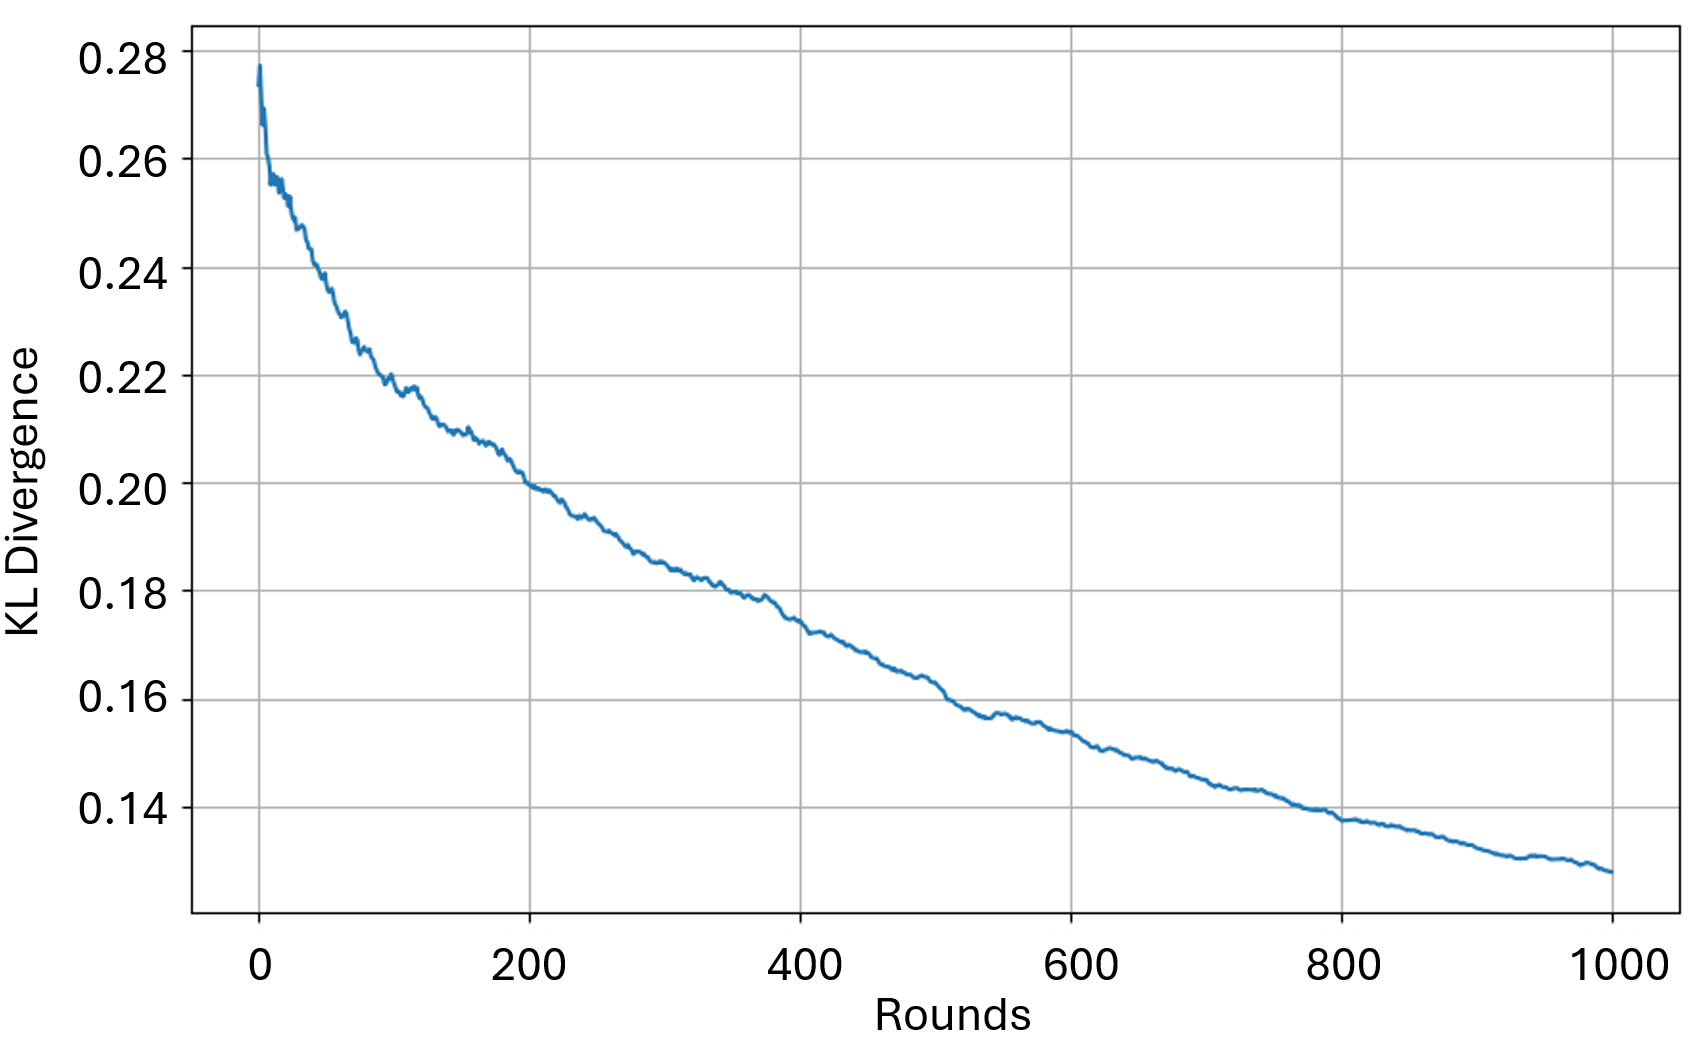
\includegraphics[width=0.30\textwidth]{paper_rq3_fig5_a.png}&
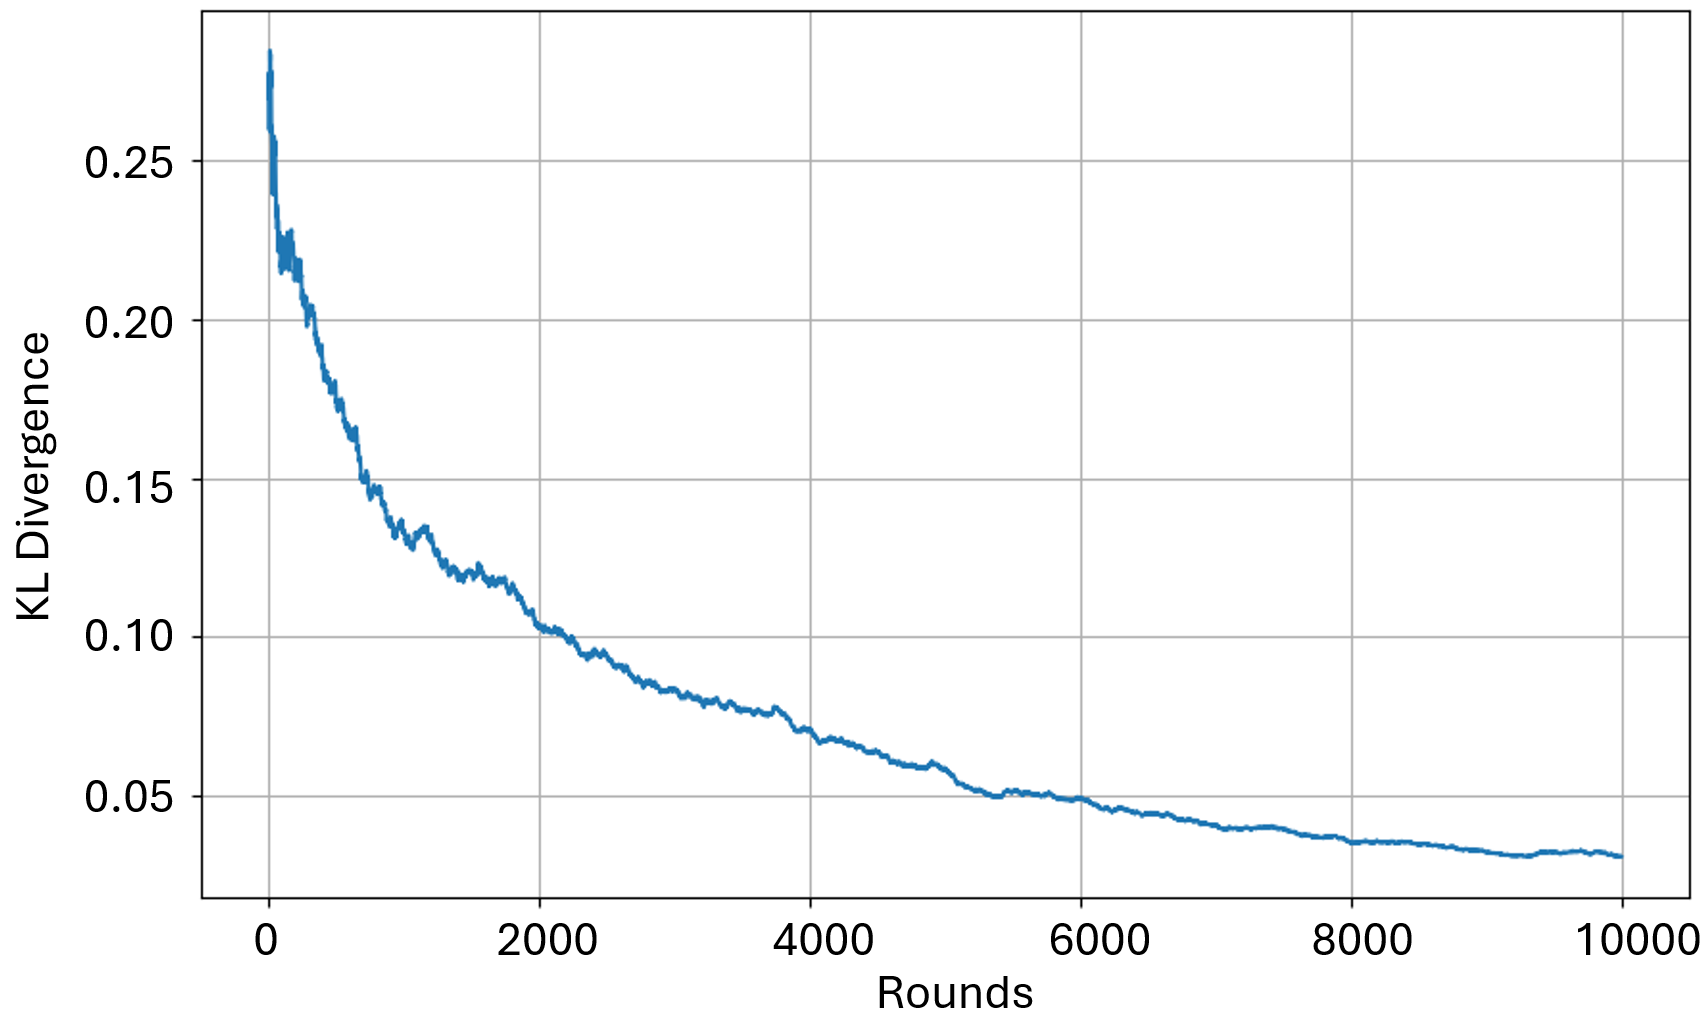
\includegraphics[width=0.30\textwidth]{paper_rq3_fig5_b.png}&
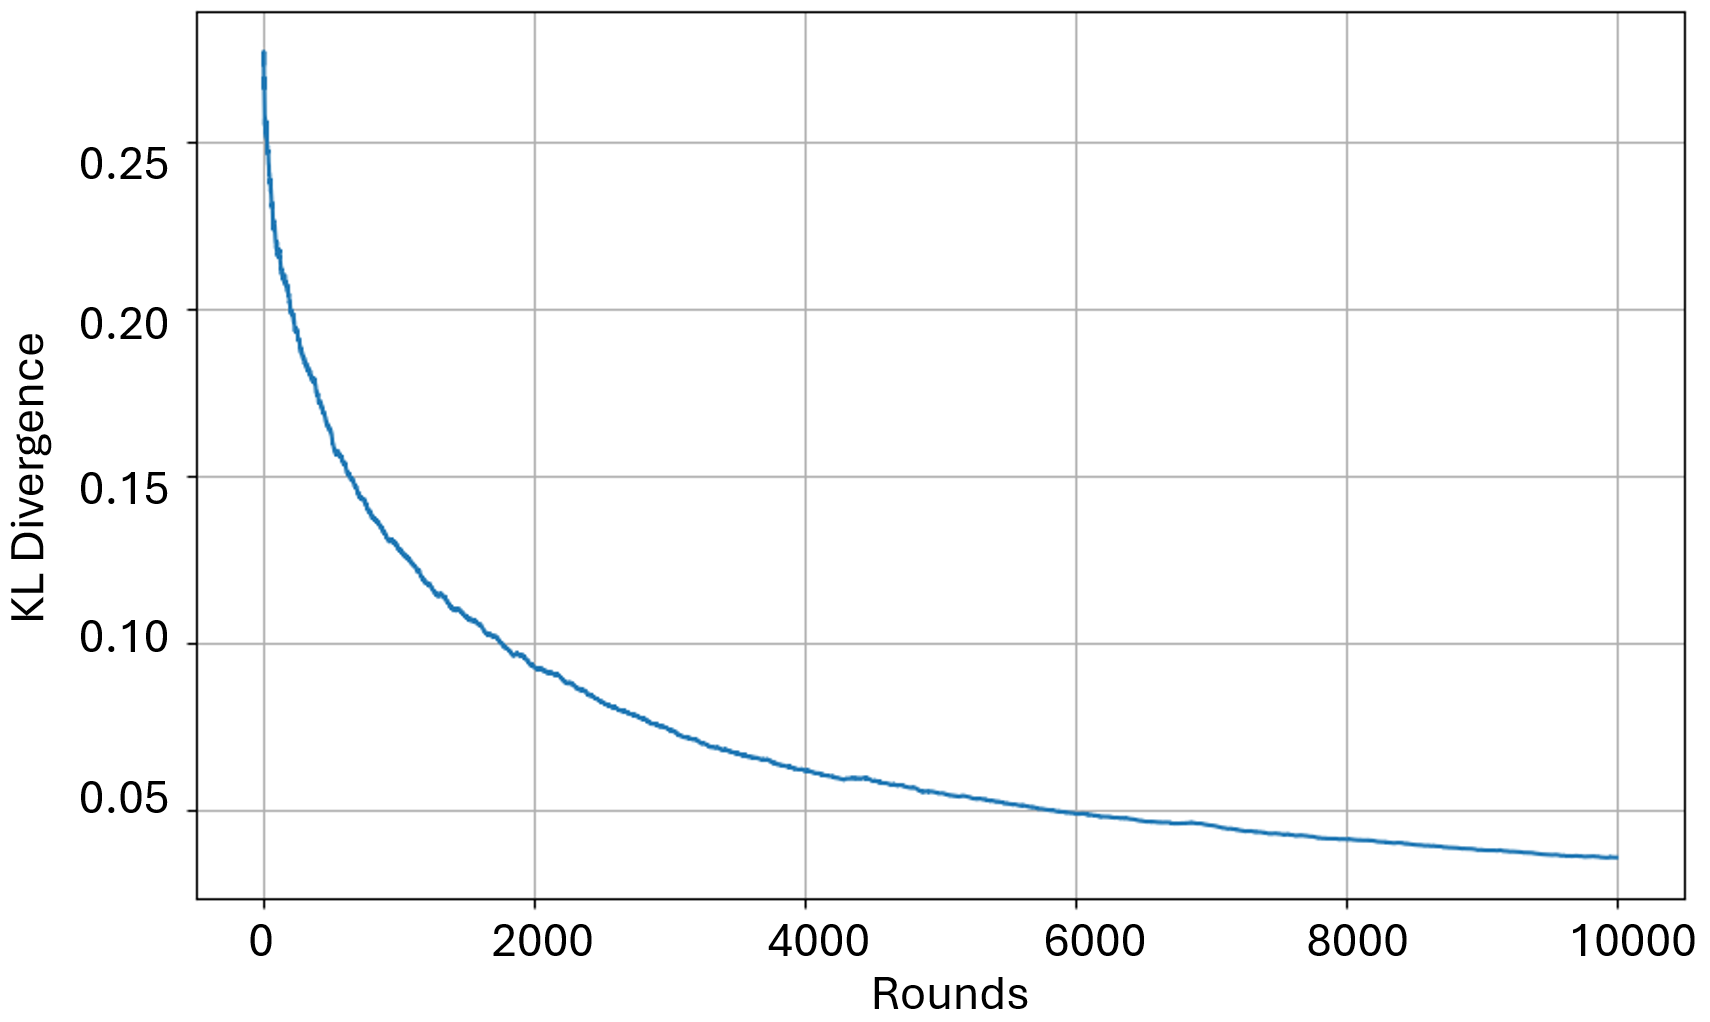
\includegraphics[width=0.30\textwidth]{paper_rq3_fig5_c.png}\\
(a) 批量 100，1000 轮&(b) 批量 10，10000 轮&(c) 批量 100，10000 轮
\end{tabular}
\caption{原论文 Figure 5 的三个 KL 曲线面板；正文使用学习率 $1/\sqrt t$。}
\label{fig:paper-rq3}
\end{figure}
作者观察到 KL 低于约 0.025 并继续下降；更激进学习率收敛更快但不稳定；增大批量可平滑波动。

\subsection{本项目怎样缩减复现 RQ3}
项目构造一个透明的有限 Markov 环境：
\begin{itemize}
  \item 10 个质量状态，最长 15 轮；初始质量只落在前三档；
  \item 每轮以 52\% 概率停留、34\% 概率升一档、14\% 概率升两档；
  \item 五类估值为 $v_i(q)=a_i\sqrt q$，其中 $a_i\in\{0.20,0.30,0.40,0.50,0.55\}$；发现成本为 0.018；
  \item 用最优停止 DP 的精确前向状态传播计算各类型的停止似然，不引入 Monte Carlo 估计误差；
  \item 五类平均停止轮次约为 1.0、4.0、7.2、10.2、12.6，最小成对 $L_1$ 距离约 0.656，显式满足可识别性；
  \item 5 种真实先验、3 种学习率、批量 10/100、5 个种子、1000 轮，共 $5\times3\times2\times5=150$ 条学习运行。
\end{itemize}

\subsection{复现结果及准确解读}
\begin{figure}[H]
\centering
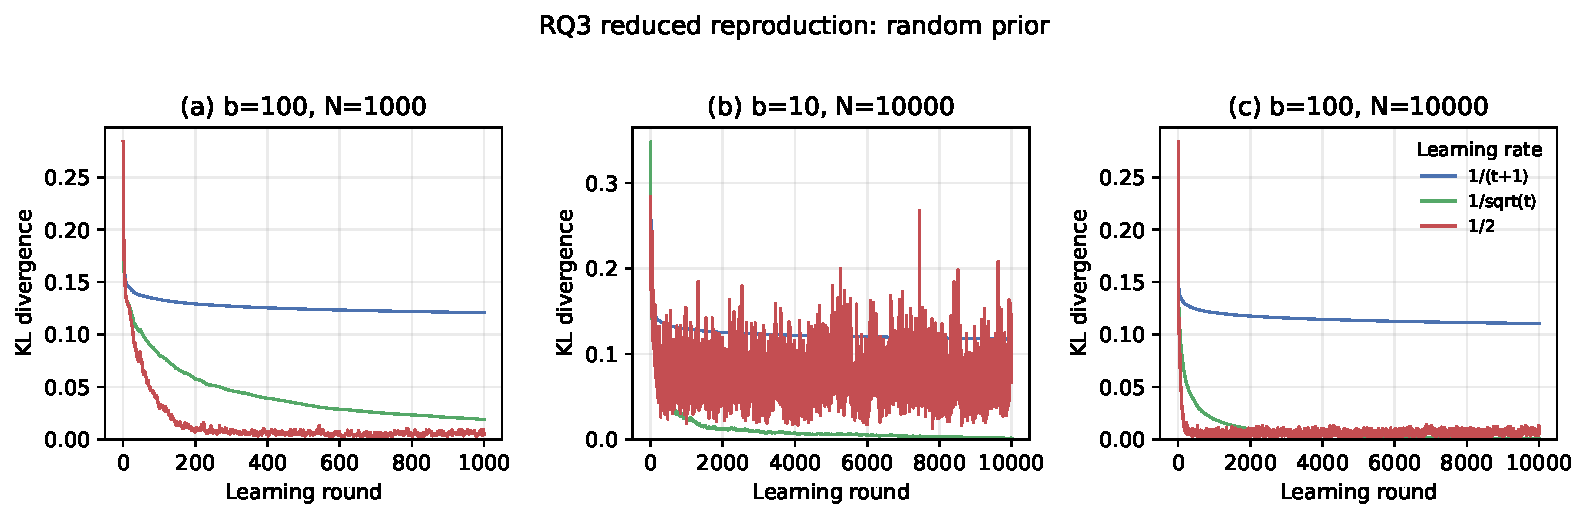
\includegraphics[width=0.98\textwidth]{rq3_paper_reproduction.pdf}
\caption{RQ3 缩减复现：精确停止似然下，三种批量/轮数组合中的学习率--收敛权衡。}
\label{fig:rq3-reproduction}
\end{figure}

\begin{table}[H]
\centering
\caption{随机先验、批量 100、1000 轮的关键数字（均值 $\pm$ 标准误，5 个种子）。}
\begin{tabular}{lrrr}
\toprule
学习率 & 最终 KL & 尾部平均 KL & 尾部标准差\\
\midrule
$1/(t+1)$ & $0.12083\pm0.00371$ & 0.12108 & \textbf{0.00015}\\
$1/\sqrt t$ & $0.01926\pm0.00139$ & 0.02008 & 0.00062\\
$1/2$ & \textbf{$0.00495\pm0.00169$} & \textbf{0.00607} & 0.00387\\
\bottomrule
\end{tabular}
\end{table}

\begin{enumerate}
  \item \key{只看最终点：}常数 $1/2$ 最低，说明它适应很快。
  \item \key{看尾部波动：}$1/2$ 的标准差 0.00387，约为 $1/(t+1)$ 的 26 倍，因此不能只说它“最好”。
  \item \key{看速度--稳定性：}$1/\sqrt t$ 最终误差接近常数率，但波动小一个数量级，是更均衡的选择。
  \item \key{看批量：}批量 10 时，常数 $1/2$ 在五种先验上的平均最终 KL 约 0.1732，尾部标准差约 0.0459，明显比批量 100 不稳定。
\end{enumerate}

\begin{takeaway}
RQ3 复现了论文的定性结论：学习能够收敛；激进学习率快但抖；大批量能抑制抽样噪声。$1/\sqrt t$ 是较稳妥的折中，但不是一个对所有市场都最优的定理。
\end{takeaway}

\subsection{RQ3 代码与复现入口}
\begin{itemize}
  \item 学习算法：\path{src/automl_market/learning.py}
  \item 停止 DP：\path{src/automl_market/market.py}
  \item 实验环境：\path{src/automl_market/paper_experiments.py}
  \item 逐运行结果：\path{results/tables/rq3_paper_reproduction.csv}
\end{itemize}
\begin{lstlisting}[language=bash]
conda activate automl-market
make paper-experiments
\end{lstlisting}

\section{上台时怎样把两部分串起来}
建议用“\key{问题--算法--实验--边界}”四步讲每个 RQ，而不是逐条读参数：
\begin{enumerate}
  \item RQ1 问组合太多时怎样减少训练；Algorithm 2 用增强搜索加 Exp3，每轮只训练一个模型。
  \item AUC 和达到 95\% oracle 的训练数显示前期更高效；但 Data-All 终点略高，对 Data-Alt 没有显著优势。
  \item 转场：发现引擎产生性能轨迹，买家在轨迹上停止；停止时间本身又暴露类型信息。
  \item RQ3 预计算各类停止似然，做 Bayes 后验，再用学习率平滑。
  \item KL 下降说明学习有效；三种学习率展示速度--稳定性权衡；批量 100 更平滑。
  \item 最后强调可识别性和缩减复现边界。
\end{enumerate}

\section{建议的 7--8 分钟讲述稿}
\subsection*{RQ1（约 3.5 分钟）}
“RQ1 问的是平台能否用较少训练找到高质量的数据增强和模型组合。难点是增强集合很大，而且每个增强如果再训练全部模型，开销会乘上模型数。论文的 Algorithm 2 用两层搜索：Metam 风格方法提出增强，Exp3 把模型当作 bandit 的臂，每轮只抽一个模型训练。概率由历史权重和均匀探索组成，重要性加权奖励用来修正只观察一只臂造成的偏差。

原文在 69K 个 NYC 数据集和 1000 个任务上比较四种方法，报告 Bandit 在更短时间达到更高效用。由于数据和完整代码未公开，我们在 UCI Wine Quality 上构造 60 个公开任务，以模型训练次数作为预算。相比 Data-All，Bandit 的发现曲线 AUC 在分类和回归上分别高 0.00794 和 0.00335，配对区间不跨 0；达到 95\% oracle 增益所需训练减少约 30.3\% 和 27.5\%。但 60 次预算终点仍是 Data-All 略高，而且 Bandit 与 Data-Alt 的区间跨 0。因此准确结论是 Bandit 更早接近最优，而不是所有指标都无条件最好。”

\subsection*{RQ3（约 3.5 分钟）}
“RQ3 问平台能不能从买家的停止时间学习真实类型分布。不同类型的估值不同，所以面对相同轨迹和价格会在不同轮次停止。Algorithm 1 先根据最优停止策略预计算每种类型在各轮停止的概率，观察实际停止轮次后用 Bayes 公式得到后验，再以学习率把后验平滑到当前先验。如果一轮有多个买家，就先平均后验。

我们比较 $1/(t+1)$、$1/\sqrt t$ 和常数 $1/2$。前者最稳定但很快变得保守，常数率最快但持续受噪声影响，$1/\sqrt t$ 位于中间。复现构造五类平均停止轮次从约 1.0 到 12.6 的买家。在随机先验、批量 100 下，最终 KL 分别约为 0.12083、0.01926、0.00495；但常数率的尾部波动约 0.00387，是保守率的 26 倍。批量降到 10 时常数率明显失稳。所以结论不是常数率绝对最好，而是更激进的学习率更快，大批量更平滑，$1/\sqrt t$ 给出较好的折中。这个结论依赖可识别性，而且我们的停止似然来自透明合成环境。”

\subsection*{收束（约 30 秒）}
“RQ1 和 RQ3 分别闭合了市场链条的两端：Data-Bandit 低成本产生性能轨迹，买家的停止行为又让平台逐步学习市场先验。两组缩减实验都复现了论文的主要定性现象，同时保留了公开数据和合成设置带来的边界。”

\section{老师可能追问什么}
\begin{longtable}{>{\bfseries\raggedright\arraybackslash}p{0.28\textwidth}>{\raggedright\arraybackslash}p{0.65\textwidth}}
\toprule
可能问题 & 建议回答\\
\midrule
\endfirsthead
\toprule
可能问题 & 建议回答\\
\midrule
\endhead
为什么 Bandit 终点不如 Data-All，还说它有效？ & 它的目标是有限搜索成本下更早找到好方案。AUC 和达到 95\% oracle 的训练数刻画前期效率；预算足够时，训练全部组合的 Data-All 理应更有机会达到 oracle。\\
为什么不用普通 bandit？ & 每轮增强不同，模型奖励随输入数据变化，不满足固定随机奖励假设；Exp3 面向对抗式或非平稳序列，并保留显式探索。\\
重要性加权为什么除以抽样概率？ & 只观察被选模型的奖励。除以抽样概率可校正不同臂被观察频率不同造成的偏差；小概率事件得到更大修正。\\
为什么测试效用可以画成搜索曲线？ & 搜索和选择只使用验证分数；测试分数仅报告“验证集当前选中的方案”，不反馈给算法，因此没有直接测试泄漏。\\
RQ1 为什么不用运行秒数？ & 原始硬件、NYC 数据池和 TPOT 环境不可复刻。训练次数是透明、跨机器稳定的成本代理，但不能与原图秒数逐点比较。\\
Bayes 更新为什么还要学习率？ & 单次后验噪声大，直接替换先验会过度响应当前样本。凸组合控制每轮更新幅度，使速度和稳定性可调。\\
常数 $1/2$ 最终 KL 最小，为什么推荐 $1/\sqrt t$？ & 最后一点不是全部。常数率尾部波动大，小批量时明显失稳；$1/\sqrt t$ 的误差接近常数率但稳定得多。\\
可识别性不满足怎么办？ & 仅凭停止时间无法区分这些类型，应引入更多行为信号或价格实验；若始终不可区分，按论文思路合并为一个有效类型。\\
RQ3 与定价有什么关系？ & 学到的先验 $\mu$ 决定平台对不同类型收入的加权，进而影响最优价格；Theorem 5.2 还说明估计误差小时收入损失也线性受控。\\
这是原论文的完全复现吗？ & 不是。RQ1 使用公开 UCI 数据替代 NYC 数据池，RQ3 使用透明合成 Markov 环境。我们复现算法语义和定性结论，不声称逐点重现 Figure 3/5。\\
\bottomrule
\end{longtable}

\section{最终记忆卡片}
\begin{tcolorbox}[colback=LightBlue,colframe=ZJUBlue,title=RQ1,fonttitle=\bfseries]
\textbf{问题：}组合太多，训练太贵。\quad
\textbf{算法：}增强搜索 + Exp3，每轮只训练一个模型。\quad
\textbf{指标：}AUC、95\% oracle 训练数、最终效用。\quad
\textbf{结果：}前期更省 27--30\%，但 Data-All 终点略高；对 Data-Alt 只可称相当。
\end{tcolorbox}

\begin{tcolorbox}[colback=LightGreen,colframe=ZJUGreen,title=RQ3,fonttitle=\bfseries]
\textbf{问题：}不知道真实买家比例。\quad
\textbf{算法：}停止似然 + Bayes 后验 + 学习率平滑。\quad
\textbf{指标：}KL、尾部均值、尾部波动。\quad
\textbf{结果：}激进率快但抖，大批量更稳，$1/\sqrt t$ 折中；可识别性必不可少。
\end{tcolorbox}

\begin{thebibliography}{9}
\bibitem{han2023} Y. Han, S. Padmanabha, S. Wang, Z. Huang, and J. Zhao. \textit{Optimal Pricing for Data-Augmented AutoML Marketplaces}. arXiv preprint, 2023.
\bibitem{uci} P. Cortez, A. Cerdeira, F. Almeida, T. Matos, and J. Reis. Wine Quality [Dataset]. UCI Machine Learning Repository, DOI: 10.24432/C56S3T.
\end{thebibliography}
\end{document}
